% Set the author and title of the compiled pdf
\hypersetup{
	pdftitle = {\Title},
	pdfauthor = {\Author}
}


\section{Recap of COMP12111 \& COMP15111}

There material in both the {\it Fundamentals of Computer Architecture} and the
{\it Fundamentals of Computer Engineering} courses in the first year provides a
good base for the course this year. The following re-visits that material and
builds upon it.

\subsection{Datapath and Control}

From the point of view of the CPU all data is of a fixed size, the length of one
word. Each word is usually moved around the architecture of the computer in a
bit-parallel manner, that is to say that there are at least the same number of
wires in a bus between any two components in the system as there are bits in the
word.

The individual operations on each bit inside a word when the CPU performs an
operation on the whole word are usually identical. This results in a very
regular datapath with lots of duplicated (usually by as many times as the word
length) hardware logic.

Control logic is derived after the datapath has been conceived. It governs which
operation is performed at what time, and is different for each instruction in
the instruction set.

A typical example of control logic might be to control the enable pin on a
binary adder. The datapath will direct bits to the adder all the time, but the
control logic will determine if the result is sent forward.

\subsection{The MU0 Instruction Set Architecture}

The MU0 is a very simple 16 bit word architecture, and as a result, the
instruction set is also very simple. Each instruction can address one memory
location, and consists of four bits for the instruction (allowing sixteen
instructions to be coded) and twelve bits for the memory address as illustrated
in Figure~\ref{instruction}. Since we can only store twelve bits of memory
address in the instruction, and the architecture is very simple, the system has
$2^{12}$ words of memory, which is equivalent to \SI{8}{\kilo\byte}.

\begin{figure}[ht!]
  \centering
  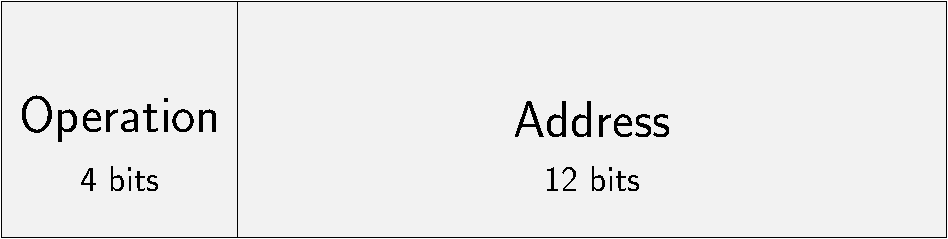
\includegraphics[width=90mm]{diagrams/instruction.pdf}
  \caption{A generic MU0 instruction}
  \label{instruction}
\end{figure}

The MU0 has two programmer visible registers, the Program Counter and the
Accumulator. The Program Counter stores the address in memory of the next
instruction to be executed, thus being twelve bits long. The Accumulator is
sixteen bits long, and stores the result of the last arithmetic operation.

The instructions that the MU0 understands are listed in
Table~\ref{instruction_set}.

\begin{table}[ht!]
  \centering
  \begin{tabular}{|c|c|c|}
    \hline
    {\bf Op Code} & {\bf Mnemonic} & {\bf Description}\\ \hline
    0 & LDA $[op]$ & $[op] \rightarrow Acc$\\ \hline
    1 & STO $[op]$ & $Acc \rightarrow [op]$\\ \hline
    2 & ADD $[op]$ & $Acc = Acc + [op]$\\ \hline
    3 & SUB $[op]$ & $Acc = Acc - [op]$\\ \hline
    4 & JMP $[op]$ & $PC = S$\\ \hline
    5 & JGE $[op]$ & If $Acc >= 0$ then $PC = S$\\ \hline
    6 & JNE $[op]$ & If $Acc \not= 0$ then $PC = S$\\ \hline
    7 & STP & Stop\\ \hline
  \end{tabular}
  \caption{The MU0 instruction set}
  \label{instruction_set}
\end{table}

\subsection{Maintaining Processor State}

If the execution cycle of the MU0 was somehow disrupted, say because of an
interrupt call, it would be handy to save the state of the processor before
switching to a different task (e.g. running the interrupt handler).

The way to do this is to save the registers in memory, doing the other task, and
then reloading them when it's time to resume execution of the program.

\subsection{The Fetch Execute Cycle}

The fetch-execute cycle describes how a CPU executes instructions. First, the
next instruction is fetched from memory (at the address pointed to by the PC),
then the instruction is executed. Since some instructions access memory (such as
load and store), and we can only do one memory access per clock cycle, one
fetch-execute cycle takes two clock cycles, one for fetching, and one for
execution.

\subsubsection{Fetching instructions}

Fetching is an operation that is the same for all instructions. First memory
addressed by the PC is read and stored into the Instruction Register (IR). This
is a 16 bit internal register that isn't visible to programmers. Once this has
occurred, the PC is incremented. This means that the RAM must be able to send a
word directly to the instruction register, so a datapath must be in place to
allow this.

\subsubsection{Executing instructions}

It is obvious that different instructions will have different paths of execution
within the processor, and will have different effects on components within the
system.

\paragraph{{\tt JMP}} In order to execute the {\tt JMP} instruction, the last
twelve bits are read from the instruction register and transferred over to the
PC. This means that there must be a datapath from the bottom twelve bits of the
IR to the PC.

\paragraph{{\tt STA}} When {\tt STA} is executed, the bottom twelve bits in the IR
are used direct the contents of the accumulator to a location in memory. To do
this, we need a datapath from the bottom twelve bits of the IR to the part of
the RAM that takes addresses, and from the PC to the part of the RAM that takes
data.

\paragraph{{\tt ADD}} To perform the {\tt ADD} instruction, we need to fetch the
bottom twelve bits of the IR and send it to the RAM. The result should be fed
into the adder along with the contents of the accumulator. The result of the
calculation should be sent to the accumulator. To do this, we need datapaths
from the accumulator to the ALU, the RAM to the ALU and finally from the ALU to
the accumulator.

\paragraph{Control Signals} whenever two separate components within the system
interact. For example, every time the CPU loads a word from the RAM, a control
signal must be sent to say `load', and every time the {\tt ADD} command it
executed, the ALU must be sent a control signal to say `add' as opposed to
subtract or shift.

\paragraph{Timing} Timing is very important when executing the instructions. If
the result of a load from RAM hasn't yet returned, but the control signal to the
ALU to add is sent, then the wrong result will almost certainly occur! In order
for everything to run smoothly, the critical path for each operation must be
worked out, and time allowed for signals to propagate through even the longest
critical path.

\subsubsection{Deriving the datapaths from the operation of instruction}

In order to produce a working processor, we need to look at all the instructions
that can be executed by the processor, and examine what datapaths and control
signals they require to work. Only when we have this information can we begin to
actually design the hardware on the CPU.

\marginpar{Note that data going to one destination can only go to one source, so
if you want multiple components to be able to send data to one other component,
then you must use a multiplexer with control signals in order to achieve this.}

\subsection{Control Signals}

The purpose of control signals is to make each component within the CPU function
as intended for each specific instruction. Control signals include:

\begin{itemize}
  \item Enable write for registers
  \item Enable write for memory
  \item Enable read for memory
  \item Multiplexer input select
  \item ALU actions (add, subtract, bypass)
\end{itemize}

Sometimes, one component (such as the ALU) may have control inputs that can be
represented by more than two states (add, bypass, subtract). If this is the
case, then multiple wires (a bus) is used to specify its action.

The first lab in the course shows the control signals sent for each instruction,
the solution for which is shown in Tables~\ref{lab:1:fetch} and
\ref{lab:1:execute}.

\begin{table}[!ht]
  \centering
    \begin{tabular}{|l|l|l|}\hline
    En\_IR  & 1 &(enable write to IR)\\ \hline
    En\_PC  & 0 &(enable write to PC)\\ \hline
    En\_ACC & X &(enable write to ACC)\\ \hline
    \hline
    byp & X &(ALU action: bypass)\\ \hline
    add & X &(ALU action: add)\\ \hline
    sub & X &(ALU action: subtract)\\ \hline
    \hline
    Ren & 1 &(RAM action: Read)\\ \hline
    Wen & 0 &(RAM action: Write)\\ \hline
    addr\_Mux& 1  &(RAM address = PC, otherwise IR.S)\\ \hline
  \end{tabular}
  \caption{The control signals in the MU0 fetch phase}
  \label{lab:1:fetch}
\end{table}

\begin{table}[!ht]
  \centering
  \begin{tabular}{|l|l|l|l|l|l|l|l|}\hline
      & lda & sta & add & sub & stp & jump  & no jump\\ \hline
    \hline
    En\_IR   & 0  & 0 & 0 & 0 & 0 & 0 & 0 \\ \hline
    En\_PC   & 0  & 0 & 0 & 0 & 0 & 1 & 0 \\ \hline
    En\_ACC  & 1  & 0 & 1 & 1 & 0 & 0 & 0 \\ \hline
    \hline
    byp      & 1  & X & 0 & 0 & X & X & X \\ \hline
    add      & 0  & X & 1 & 0 & X & X & X \\ \hline
    sub      & 0  & X & 0 & 1 & X & X & X \\ \hline
    \hline
    Ren      & 1  & 0 & 1 & 1 & 0 & 1 & 0 \\ \hline
    Wen      & 0  & 1 & 0 & 0 & 0 & 0 & 0 \\ \hline
    addr\_Mux& 0  & 0 & 0 & 0 & X & 0 & 1 \\ \hline
  \end{tabular}
  \caption{The control signals in the MU0 execute phase}
  \label{lab:1:execute}
\end{table}

\section{What does an Operating System do?}

The job of an operating system varies from system to system but on general, it
is responsible for managing the resources of the system (including dealing with
concurrency, security etc) and abstracting the implementation of the system from
the running programs (such as what exact components are being utilised).

\subsection{Processes}

A process is a program that is currently running on the system. It consists of a
Thread (a set of instructions to be executed) and address space (a set of memory
locations that can be accessed by the thread). In most systems, multi-threading
is used to allow each process own multiple threads, and therefore execute in
parallel.

\marginpar{Nearly all systems have many processes running at any one time, on a
Linux system, use {\tt htop} or {\tt ps aux} to see what processes are running.}

\subsection{Address Space}

\textit{Address space} (aka memory space) is a term used to speak about a
section of memory. This could be the whole memory avalible to the system, the
memory that a specific program has access to etc.

When a program starts, it assumes that it does so from memory address {\tt 0}.
On a single process system this is okay, however this presents a problem on
systems where multiple processes run concurrently, since no two processes can
share the same memory space.

Sometimes, operating systems may even running pause programs, move them out of
memory (onto secondary memory such as hard drive) and later on swap it back in
at a different place in memory.

In both cases, a technique called {\it Relocation} is used to make every running
program able to safely assume that it has sole use of memory.

In order to facilitate relocation, operating systems abstract away the
implementation of the hardware, and instead provide a virtual machine for each
program. This enables programs to behave as though they have the whole system
to themselves, and it also lets the operating system easily stop programs
interfereing with eachother (such as providing disjoint memory spaces for each
program).

\subsection{Modes of operation}

It is often nececarry to prevent some programs from executing some operations,
such as manipulating memory, or allocating CPU time. In order to achieve this,
operating systems nearly always implement different `modes' of operation that
processes can run under. The two most common modes are \textit{user} and
\textit{system}.

All the processes owned by the operating system will run under system mode,
which is very permissive and lets programs perform operations with the
potential for misuse. Programs that the user might run are usually executing
under user mode. User mode is less permissive, and restricts certain
operations, yet the restricted operations aren't usually required for normal
programs.

\subsubsection{System calls}

If there was an eventuality where a program needed to perform privaliged
operation that wasnn't permitted under it's current mode, then it can use a
system call to achieve the same result. The premise is that the operating
system will provide a `gatekeeper' function that will perform the requested
operation, but only after the parameters have undergone checks to ensure that
the application isn't behaving badly. The execution of the user program will
(of course) pause while the system call is running.

Lots of functions in languages that you already know might just be wrappers
around system calls, albeit often with slightly more functionality. The course
notes make a good example; \texttt{fread} in C uses the \texttt{UNIX} system
call \texttt{read}.

\section{Engineering an Operating System}

Like a lot of things in Computer Science, operating systems can often be
conceptualised as being built up of several layers. As you inspect further and
further into the OS, looking deeper into each layer as you go, the level of
abstraction decreases.

The outermost layer could be seen to be the UI, which is obviously a very
abstracted way of thinking about a computer. The kernel is probably the lowest
layer, since the details of how the hardware is managed is, also fairly
obviously, a very low level of abstraction.

Different operating systems can contain a different number of layers of
abstraction so that they are best suited to their purpose. Some operating
systems will contain little more than a microkernel, which will have the bare
minimum of logic required to keep a computer running.

Some components of an operating system are monolithic, most notably the Linux
kernel. A monolithic compoment is easier to design (especially for a kernel)
since there is less inter-process communication to worry about, and trapfalls
like race conditions can be more easily avoided when everything is running on
a single thread.

\marginpar{
  \begin{sloppypar}
    See this StackOverflow answer for an explanation (and follow the
    link to the Linus V Tanenbaum showdown on the topic):
    \texttt{http://stackoverflow.com/questions}
    \texttt{/1806585/why-is-linux-called}
    \texttt{-a-monolithic-kernel}
  \end{sloppypar}
}

I feel obliged to point out that monolithic, in this instance, refers to the
fact that the program is running under \textit{one} process that is in system
mode. It doesn't mean that the code is all in one big file, or even in one big
project, since many monolithic projects employ some degree of modularity in
the development process at least.
